\apendice{Documentación técnica de programación}

\section{Introducción}

En este apartado de la memoria, nos centraremos en la parte más técnica del trabajo, entrando a detalle sobre los cambios realizados y los problemas diversos que se han encontrado y solucionado.

Mencionaremos algunas partes que hacen referencia al servidor, teniendo en cuenta que esta parte no la hemos desarrollado, ya que lo hizo mi compañero Ignacio.

Dentro de este apartado, veremos las distintas bibliotecas que se han utilizado, las APIs, el manual del programador y tambien las pruebas realizadas. 

Cabe destacar que en este proyecto la mayor parte de desarrollo ha sido sobre la resolución de errores provocados por el cambio de versión y la antigüedad del proyecto, sin poder mostrar implementaciones nuevas con respecto a funcionalidades. Es un trabajo dedicado al mantenimiento y actualización de una aplicación que contaba con una versión y recursos con 7 años de antigüedad y por eso ha habido tanta base de problemas.

Del mismo modo que hemos hecho en algunos apartados, se mencionarán partes que ya fueron desarrolladas anteriormente y que no hayan sufrido cambios importantes.

\section{Estructura de directorios}

En este apartado vamos a enumerar distintos contenidos que tendrá el dispositivo entregable, tanto del cliente como del servidor:

\begin{itemize}
\item Cliente
 	\begin{itemize}
		\item Aplicación: dentro de esta subcarpeta tendremos el archivo TourPlanner.apk, para que pueda ser instalado en cualquier dispositivo.
		\item Código fuente: Contiene el código de la aplicación Android.
		\item Javadoc: documentación sobre la aplicación.
		\item Datos: contiene el archivo con las referencias utilizadas en el proyecto y un backup con la base de datos PostgreSQL de Burgos configurada.
		\item Máquina virtual: Dentro tendremos la máquina virtual donde estará instalado Android Studio y se podrá utilizar sin tener que hacer más instalaciones.
		\end{itemize}
		
\item Servidor
 	\begin{itemize}
		\item Aplicación: contiene el archivo osm server.war para que se pueda utilizar en cualquier momento.
		\item Código fuente: Contiene el código fuente de la aplicación servidor.
		\item Javadoc: Contiene la documentación de la aplicación servidor.
		\item Datos: Archivo con las referencias utilizadas en el proyecto y un backup con la base de datos PostgreSQL de Burgos configurada.
		\item contiene la máquina virtual del servidor configurada para ser utilizada.
		\end{itemize}
		
\item Documentación Memoria
 	\begin{itemize}	
		\item PDF: Contiene la memoria en formato PDF.
		\item Latex: Contiene la memoria en formato de latex.
		\end{itemize}
		
\item Software
 	\begin{itemize}
		\item Esta carpeta contendrá los distintos programas que se han ido utilizando en el desarrollo de la aplicación.
		\end{itemize}		
\end{itemize}

\section{Manual del programador}

Dentro de este apartado veremos todo el proceso de desarrollo que se ha realizado en el proyecto, explicando los cambios, mejoras y arreglos sobre el mismo. Lo dividiremos en distintos puntos, ya que es necesario cubrir todos los aspectos que hacen referencia al desarrollo del código y de la aplicación.

Antes de comenzar, cabe destacar que en este proyecto se ha tratado de mejorar el código de una aplicación con una antigüedad de 7 años, actualizándola a versiones compatibles con los dispositivos de hoy en día y a su vez tratando de que sea lo más estable posible. Ha habido funcionalidades que no se han podido actualizar tal y como estaban desarrolladas, por lo que se mencionarán para un futuro desarrollo.

\subsection{Modificaciones sobre la estructura}

En este pequeño apartado mencionaremos las modificaciones que ha sufrido la estructura dentro de la herramienta de desarrollo, partiendo de la base de que la herramienta en sí es distinta y consideramos que para este propósito Android Studio consigue una estructura más clara y sencilla, donde se pueden localizar mejor las distintas partes de las que está compuesta la aplicación, porque está organizada de forma mas homogénea.

En el proyecto anterior contábamos con una estructura como la siguiente:

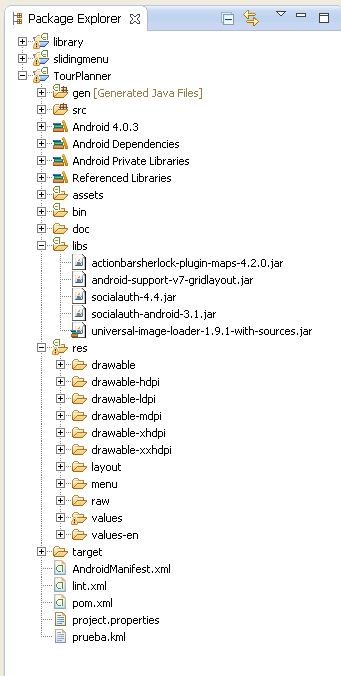
\includegraphics[width=\textwidth]{androidAnterior.jpg}

Aquí se puede observar que hay 3 carpetas principales:

\begin{itemize}
\item Tourplanner, la cual hace referencia a la aplicación. Dentro de esta carpeta esta la mayor parte del código de desarrollo y tambien se hace referencia a librerías y recursos.
\item SlidingMenu, que en este proyecto es la biblioteca utilizada para generar el menú lateral con el cuenta la aplicación. Como se puede ver es necesario que esté implementada de manera individual, en vez de ser importada como el resto de librerias y también tiene código dentro de sus subcarpetas.
\item libraries, que hace referencia a las librerias que estan utilizando en el proyecto, excepto SlidingMenu por lo que acabamos de ver.
\end{itemize}

Comparando esta estructura con la que tenemos actualmente podremos ver bastantes diferencias:

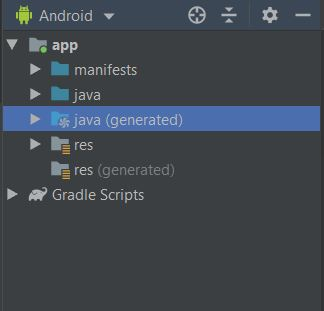
\includegraphics[width=\textwidth]{androidNuevo.jpg}

En este caso, podemos ver una estructura mas sencilla, ya que sólo contamos con una carpeta principal de la que aparecen el resto de elementos. 

La carpeta java, que será donde se encuentre todo el código de desarrollo de la aplicación. No tendremos que estar desplazandonos entre otros directorios para poder encontrar código, ya que estará al completo aquí.

\subsubsection{Gradle Scripts}

Por otro lado, el apartado de Gradle Scripts es algo que Android Studio implementa por defecto en todos los proyectos, y es una herramienta muy útil cuando se trabaja con un numero considerable de librerias, pudiendo manejar a la perfección qué se está importando para que sea utilizado, así como las versiones en las que lo implantamos.

El hecho de poder manejar las versiones de esta manera nos permite poder mantener la aplicación lo más actualizada posible continuamente, ya que además el propio Software nos advertirá siempre que tengamos versiones de repositorios para los cuales ya hay otras más nuevas. Esto ayuda a mantenerse siempre lo más alejado posible de trabajar con "bujs" y errores de desarrollo de los propios repositorios, ya que suele ser lo que se corrige cuando se actualiza el Software.

El fichero más importante del apartado de Gradle será el llamado "build.gradle", ya que será con el que podremos añadir repositorios y bibliotecas para que despues podamos implementar en el código.

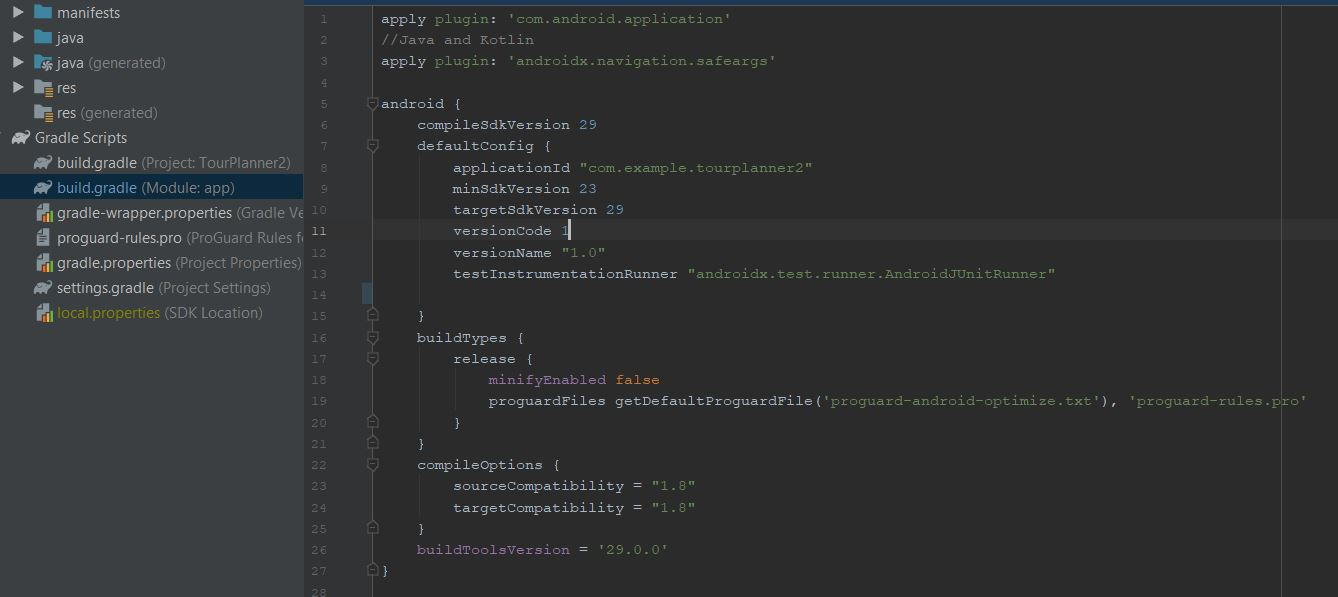
\includegraphics[width=\textwidth]{gradle1.jpg}

Como se puede observar, aquí configuraremos la versión de sdk con la que estamos trabajando y la versión mínima con la que podremos hacer funcionar la aplicación. La versión mínima será la API 23, como se indica en esta configuración y la versión objetivo que se menciona aquí también será la API 29, que es la última con la que cuenta Android. Nuestra aplicación funcionará para dispositivos con versión Android 6.0 (API 23) o superior.

Por último podemos ver cómo nos recomienda Android que mantengamos actualizado nuestro software y repositorios, ya que en el momento que alguno de ellos tiene una versión disponible superior, nos los marcará:

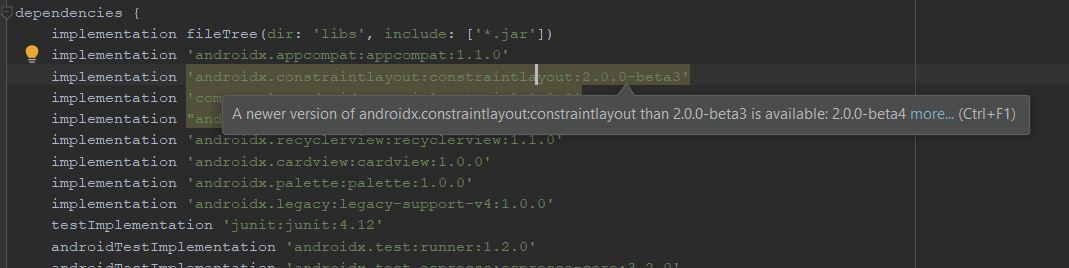
\includegraphics[width=\textwidth]{gradleVersion.jpg}

\subsection{Modificaciones importantes sobre bibliotecas}

Como ya hemos mencionado en otros apartados de la memoria, se han realizado muchas modificaciones sobre las librerías que estaban siendo utilizadas previamente y que, por desgracia, han quedado totalmente obsoletas. Esto nos ha llevado a intentar descubrir todas las novedades que se han ido implementando en el software de Android desde el desarrollo del anterior proyecto.

\subsubsection{Cambio de SlidingMenu}

Uno de los primeros descubrimientos que nos vimos obligados a realizar fue el de una nueva herramienta par obtener el menú "deslizante" con el que contaba la aplicación, o al menos un nuevo menú que cumpliera la función que ya cumplía previamente SlidingMenu.

Esto se debe a que la librería de SlidingMenu quedo obsoleta, y no se siguió desarrollando soporte para la misma a lo largo de las nuevas versiones, por lo que al intentar utilizarla en Android Studio con la versión para la API 23, ésta no era reconocida.

De esta forma, hemos desarrollado el nuevo menú de la aplicación, utilizando una versión más estándar proveniente de Android, lo cual nos asegurará más soporte de cara a futuro y es mucho menos probable que tenga que ser sustituida por completo en una futura versión. El menú en cuestión es NavigationMethod y es una funcionalidad de la biblioteca de androidx, la cual ha sido utilizada en muchas partes de este proyecto. Éste menú nos ofrece una funcionalidad muy parecida a lo que ya nos encontrábamos antes, pero mejorando la eficiencia y la visualización, siendo esta última bastante más parecida a la que nos podemos encontrar en cualquier dispositivo que utilice Android. Esto también ayuda a la accesibilidad de cara al usuario.

La interfaz del menú que teníamos antes era de esta forma:

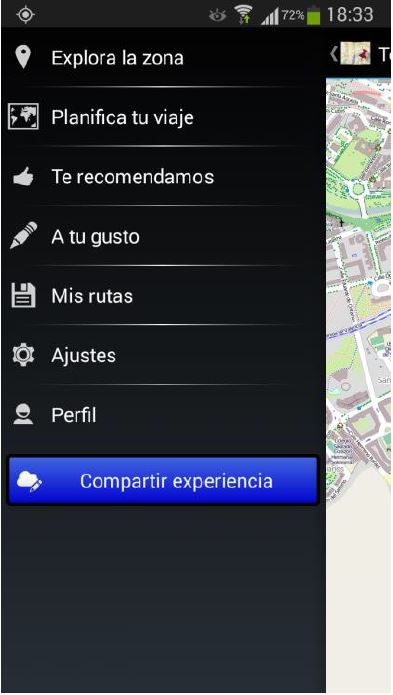
\includegraphics[scale=1]{interfazVieja.jpg}

La interfaz del menú que tenemos ahora es de la forma:

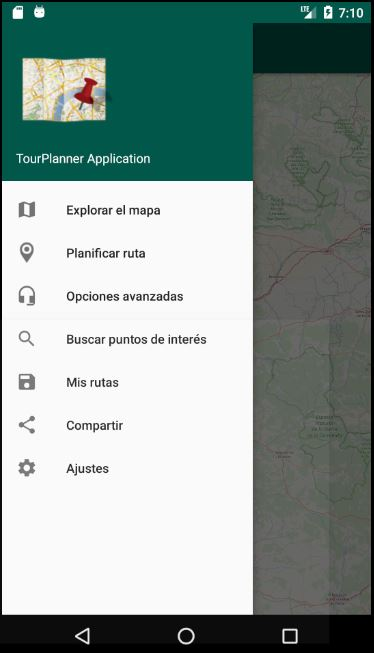
\includegraphics[scale=1]{interfazNueva.jpg}

Como podemos ver, hay un cambio considerable, tanto en facilidad a la hora de visualizarlo, como de desarrollarlo en código, ya que implementar este menú, al ser un estándar de Android, nos resulta una tarea más accesible y en caso de tener dudas, también es mas sencillo conseguir documentación al respecto. Estas son las ventajas que nos ofrece estar utilizando repositorios estándar para Android.

Las dos bibliotecas que han sustituido a SlidingMenu han sido:

\begin{itemize}
\item NavigationMethod, y los métodos que implementa.
\item Android.view.Menu
\end{itemize}

También los colores es algo en lo que se ha puesto cierta atención a la hora de desarrollar este menú y el resto de la aplicación, ya que consideramos que la accesibilidad de una aplicación hoy en día es un valor añadido muy importante. Se ha tratado de manejar colores que faciliten a la lectura y visualización, siguiendo los estándares de accesibilidad de W3C.


 

\section{Compilación, instalación y ejecución del proyecto}

\section{Pruebas del sistema}
